% THIS IS SIGPROC-SP.TEX - VERSION 4.1
% WORKS WITH V3.2SP OF ACM_PROC_ARTICLE-SP.CLS
% APRIL 2009
%
% It is an example file showing how to use the 'acm_proc_article-sp.cls' V3.2SP
% LaTeX2e document class file for Conference Proceedings submissions.
% ----------------------------------------------------------------------------------------------------------------
% This .tex file (and associated .cls V3.2SP) *DOES NOT* produce:
%       1) The Permission Statement
%       2) The Conference (location) Info information
%       3) The Copyright Line with ACM data
%       4) Page numbering
% ---------------------------------------------------------------------------------------------------------------
% It is an example which *does* use the .bib file (from which the .bbl file
% is produced).
% REMEMBER HOWEVER: After having produced the .bbl file,
% and prior to final submission,
% you need to 'insert'  your .bbl file into your source .tex file so as to provide
% ONE 'self-contained' source file.
%
% Questions regarding SIGS should be sent to
% Adrienne Griscti ---> griscti@acm.org
%
% Questions/suggestions regarding the guidelines, .tex and .cls files, etc. to
% Gerald Murray ---> murray@hq.acm.org
%
% For tracking purposes - this is V3.1SP - APRIL 2009

\documentclass{acm_proc_article-sp}
%\usepackage{epsfig}
%\usepackage{graphicx}
\newdef{definition}{Definition}
\usepackage[
  pagebackref,
  pdfpagelabels,
  extension=pdf,
]{hyperref}
\newcommand{\secref}[1] {\hyperref[#1]{Section~\ref*{#1}}}
\newcommand{\figref}[1] {\hyperref[#1]{Figure~\ref*{#1}}}
\newcommand{\eqnref}[1] {Equation \eqref{#1}}

\begin{document}
\title{Citation Centrality and Academic Salaries}
%
% You need the command \numberofauthors to handle the 'placement
% and alignment' of the authors beneath the title.
%
% For aesthetic reasons, we recommend 'three authors at a time'
% i.e. three 'name/affiliation blocks' be placed beneath the title.
%
% NOTE: You are NOT restricted in how many 'rows' of
% "name/affiliations" may appear. We just ask that you restrict
% the number of 'columns' to three.
%
% Because of the available 'opening page real-estate'
% we ask you to refrain from putting more than six authors
% (two rows with three columns) beneath the article title.
% More than six makes the first-page appear very cluttered indeed.
%
% Use the \alignauthor commands to handle the names
% and affiliations for an 'aesthetic maximum' of six authors.
% Add names, affiliations, addresses for
% the seventh etc. author(s) as the argument for the
% \additionalauthors command.
% These 'additional authors' will be output/set for you
% without further effort on your part as the last section in
% the body of your article BEFORE References or any Appendices.

\numberofauthors{3} %  in this sample file, there are a *total*
% of EIGHT authors. SIX appear on the 'first-page' (for formatting
% reasons) and the remaining two appear in the \additionalauthors section.
%
\author{
% You can go ahead and credit any number of authors here,
% e.g. one 'row of three' or two rows (consisting of one row of three
% and a second row of one, two or three).
%
% The command \alignauthor (no curly braces needed) should
% precede each author name, affiliation/snail-mail address and
% e-mail address. Additionally, tag each line of
% affiliation/address with \affaddr, and tag the
% e-mail address with \email.
%
% Authors in alphabetical order
\alignauthor 
Michael Hirshleifer\\
       \affaddr{Computer Science \& Engineering}\\
       \affaddr{California Institute of Technology}\\
       \email{111mth@caltech.edu}
\alignauthor
Kijun Seo\\
       \affaddr{Computer Science \& Engineering}\\
       \affaddr{California Institute of Technology}\\
       \email{kijun@caltech.edu}
\alignauthor
% @@@@@@@@@ Assuming Vinayak is the surname? If not, fix order
Ramya Korlakai Vinayak\\
       \affaddr{Electrical Engineering}\\
       \affaddr{California Institute of Technology}\\
       \email{ramya@caltech.edu}
}

% There's nothing stopping you putting the seventh, eighth, etc.
% author on the opening page (as the 'third row') but we ask,
% for aesthetic reasons that you place these 'additional authors'
% in the \additional authors block, viz.
\date{8 June, 2012}
% Just remember to make sure that the TOTAL number of authors
% is the number that will appear on the first page PLUS the
% number that will appear in the \additionalauthors section.

\maketitle

\input abstract.tex

% A category with the (minimum) three required fields
\category{H.3.7}{Digital Libraries}{}
%A category including the fourth, optional field follows...
%\category{}{}[]

\terms{Measurement, Experimentation, Economics}

\keywords{Citation Network, Publication Impact, Salary} % NOT required for Proceedings

\section{Introduction}
\input intro.tex

\section{Model}
\input model.tex


\section{Data}
\label{sectionData}
\input data.tex

\section{Results and Discussion}
\subsection{Our model for analysis}

\subsubsection{Years since Ph.D.}

To decide whether the number of years since each scholar received his Ph.D. (a simple measure of seniority) is a major factor to be considered for regression, we plotted base salary versus years since Ph.D.. From \figref{figYearPhD} we find a clear correlation between base salary and seniority. Thus, let us include years since Ph.D. as a secondary regressor in our regressions.

\begin{figure}[h]
\label{figYearPhD}
\centering
%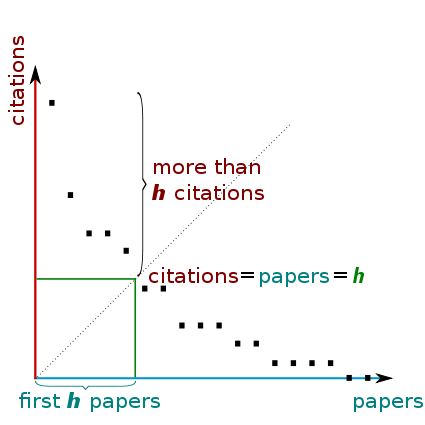
\epsfig{file=figures/hindex.eps}
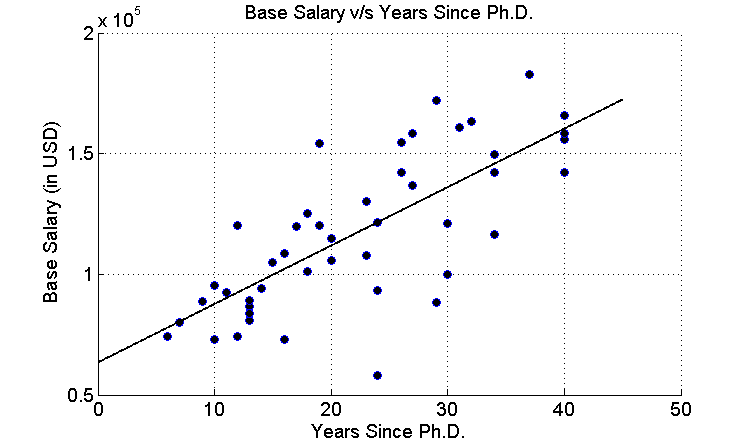
\includegraphics[width=0.5\textwidth]{figures/yrPhD.png}
\caption{Base salary plotted against years since Ph.D. shows a correlation.}
\end{figure}

This gives our generic simple linear regression model:

\begin{equation}
  \label{eqnourmodel}
  salary = \beta_0 + \beta_1 \text{Years Since Ph.D.} + \beta_2 \text{Productivity}
\end{equation}


\subsection{Results}
\input result.tex

\subsection{Discussion}
\input discuss.tex

\section{Conclusions}
\input concl.tex

%ACKNOWLEDGMENTS are optional
\section{Acknowledgments}
\input ack.tex

% The following two commands are all you need in the
% initial runs of your .tex file to
% produce the bibliography for the citations in your paper.
\bibliographystyle{abbrv}
\bibliography{ref}  % sigproc.bib is the name of the Bibliography in this case
% You must have a proper ".bib" file
%  and remember to run:
% latex bibtex latex latex
% to resolve all references
%
% ACM needs 'a single self-contained file'!
%
%APPENDICES are optional
%\balancecolumns

\end{document}
